%!TEX root = /Users/louis/Documents/PhD/Deliverables/Thesis/thesis.tex

\chapter{Analysis}
\label{Analysis}
The review presented in Chapter~\ref{LiteratureReview} highlighted challenges for identifying and managing evolution in the context of MDE, and noted that little work has explored the way in which evolution occurs in practice. This chapter explores evolution in the context of MDE by identifying and analysing examples from software engineering projects developed in a model-driven manner. The analysis presented in this chapter facilitated the identification of requirements for the thesis research, which were approached by the work presented in Chapter~\ref{Implementation}.

Figure~\ref{fig:analysis_overview} summarises the objectives of this chapter. Examples of evolution in MDE projects were located (Section~\ref{sec:locating_data}) and used to analyse existing co-evolution techniques. Analysis led to a categorisation and comparison of existing co-evolution approaches (Section~\ref{sec:analysing_existing_techniques}) and to the identification of modelling framework characteristics that restrict the way in which co-evolution can be managed (Section~\ref{subsec:modelling_framework_characteristics}). Research requirements for this thesis were identified from the analysis presented in this chapter (Section~\ref{sec:requirements_identification}).


\begin{figure}[htbp]
  \begin{center}
    \leavevmode
    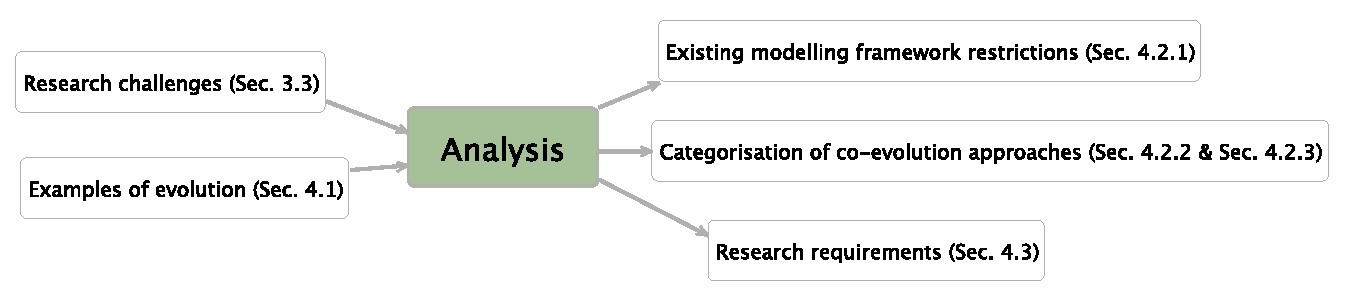
\includegraphics[width=12cm]{4.Analysis/overview.pdf}
  \end{center}
  \caption{Analysis chapter overview.}
  \label{fig:analysis_overview}
\end{figure}

Earlier in this thesis, the term \emph{modelling framework} has meant an implementation of a set of abstractions for defining, checking and otherwise managing models. The remainder of this thesis focuses on modelling frameworks used for MDE, and, more specifically, contemporary MDE modelling frameworks such as the Eclipse Modeling Framework \cite{steinberg09emf}. Throughout the remainder of this thesis, the term \emph{modelling framework} is used to mean contemporary MDE modelling frameworks, unless otherwise stated.


\section{Locating Data}
\label{sec:locating_data}
In Chapter~\ref{LiteratureReview}, three categories of evolutionary change were identified: model refactoring, synchronisation and co-evolution. Existing MDE projects were examined for examples of synchronisation and co-evolution and, due to time constraints, examples of model refactoring were not considered. The examples were used to provide requirements for developing structures and processes for evolutionary changes in the context of MDE. In this section, the requirements used to select example data are described, along with candidate and selected MDE projects. The section concludes with a discussion of further examples, which were obtained from joint research -- with colleagues in this department and at the University of Kent -- and from related work on the evolution of object-oriented programs.  

\subsection{Requirements}
The requirements used to select example data are now discussed. Requirements were partitioned into: those necessary for studying each of the two categories of evolutionary change, and common requirements (applicable to both categories of evolutionary change). MDE projects were evaluated against these requirements, and several were selected for further analysis.

\subsubsection{Common requirements}
Every candidate project needs to use MDE. Specifically, both metamodelling and model transformation must be used (requirement R1). In addition, each candidate project needs to provide historical information to trace the evolution of development artefacts (R2). For example, several versions of the project are needed perhaps in a source code management system. Finally, a candidate project needs to have undergone a number of significant changes\footnote{This is deliberately vague. Further details are given in Section~\ref{subsec:project_selection}.} (R3).

\subsubsection{Co-evolution requirements}
A candidate project for the study of co-evolution needs to define a metamodel and some changes to that metamodel (R4). In the projects considered, the metamodel changes took the form of either another version of the metamodel, or a history (which recorded each of the steps used to produce the adapted metamodel). A candidate project also needs to provide example instances of models before and after each migration activity (R5).

Ideally, a candidate project should include more than one metamodel adaptation in sequence, so as to represent the way in which the same development artefacts continue to evolve over time (optional requirement O1).

\subsubsection{Synchronisation requirements}
A candidate project for the study of synchronisation needs to define a model-to-model transformation (R6). Furthermore, a candidate project has to include many examples of source and target models for that transformation (R7). A candidate project needs to provide many examples of the kinds of change (to either source or target model) that cause inconsistency between the models (R8). 

Ideally, a candidate project should also include transformation chains (more than one model-to-model transformation, executed sequentially) (O2). Chains of transformations are prescribed by the MDA guidelines \cite{kleppe03mda}.


\subsection{Project Selection}
\label{subsec:project_selection}
Eight candidate projects were considered for the study. Table \ref{tab:candidates} shows which of the requirements are fulfilled by each of the candidates. Each candidate is now discussed in turn.

\begin{table}
	\centering
	\begin{tabular}{|c||c|c|c||c|c|c||c|c|c|c|}
		\hline
		\multirow{3}{*}{Name} & \multicolumn{10}{|c|}{Requirements} \\
		\cline{2-11}
		          & \multicolumn{3}{|c||}{Common} & \multicolumn{3}{|c||}{Co-evolution} & \multicolumn{4}{|c|}{Synchronisation} \\
		\cline{2-11}
		          & R1 & R2 & R3 & R4 & R5 & O1 & R6 & R7 & R8 & O2 \\
		\hline
		GSN       & x  &    &    & x  &    &    &    &    &    &    \\
		\hline
		OMG       & x  &    &    & x  &    &    & x  &    &    &    \\
		\hline
		Zoos      & x  & x  &    & x  &    &    &    &    &    &    \\
		\hline
		MDT       & x  & x  &    & x  &    & x  &    &    &    &    \\
		\hline
		MODELPLEX & x  & x  & x  & x  &    & x  & x  & x  &    &    \\
		\hline
		FPTC      & x  & x  & x  & x  & x  &    &    &    &    &    \\
		\hline
		xText     & x  & x  & x  & x  & x  & x  & x  & x  &    & x  \\
		\hline
		GMF       & x  & x  & x  & x  & x  & x  & x  & x  &    & x  \\
		\hline
	\end{tabular}
	\label{tab:candidates}
	\caption{Candidates for study of evolution in existing MDE projects}
\end{table}

\subsubsection{GSN}
\label{par:gsn}
Georgios Despotou and Tim Kelly, members of this department's High Integrity Systems Engineering group, are constructing a metamodel for Goal Structuring Notation (GSN). The metamodel has been developed incrementally. There is no accurate and detailed version history for the GSN metamodel (requirement R2). \textbf{Suitability for study:} Unsuitable.

\subsubsection{OMG}
\label{par:omg}
The Object Management Group (OMG)\footnote{\url{http://www.omg.org}} oversees the development of model-driven technologies. The Vice President and Technical Director of OMG, Andrew Watson, references the development of two MDE projects in \cite{watson08mdahistory}. Personal correspondence with Watson ascertained that source code is available for one of the projects, but there is no version history. \textbf{Suitability for study:} Unsuitable.

\subsubsection{Zoos}
\label{par:zoos}
A zoo is a collection of metamodels, authored in a common metamodelling language. Two zoos were considered (the Atlantic Zoo and the AtlantEcore Zoo\footnote{Both have since moved to: \url{http://www.emn.fr/z-info/atlanmod/index.php/Zoos}}), but neither contained significant metamodel changes. Those changes that were made involved only renaming of meta-classes (trivial to migrate) or additive changes (which do not affect conformance, and therefore require no migration). \textbf{Suitability for study:} Unsuitable.

\subsubsection{MDT}
The Eclipse Model Development Tools (MDT)\footnote{\url{http://www.eclipse.org/mdt}} provides implementations of industry-standard metamodels, such as UML2 \cite{uml212} and OCL \cite{ocl2}. Like the metamodel zoos, the version history for the MDT metamodels contained no significant changes. \textbf{Suitability for study:} Unsuitable.

\subsubsection{MODELPLEX}
Jendrik Johannes, a Research Assistant at TU Dresden, has made available work from the European project, MODELPLEX\footnote{TODO: Ask Richard for grant number. \url{http://www.modelplex.org/}}. Johannes's work involves transforming UML models to Tool Independent Performance Models (TIPM) for simulation. Although the TIPM metamodel and the UML-to-TIPM transformation have been changed significantly, no significant changes have been made to the models. The TIPM metamodel was changed such that conformance was not affected. \textbf{Suitability for study:} Unsuitable.

\subsubsection{FPTC}
Failure Propagation and Transformation Calculus (FPTC), developed by Malcolm Wallace in this department, provides a means for reasoning about the failure behaviour of complex systems. In an earlier project, Richard Paige and the author developed an implementation of FPTC in Eclipse. The implementation includes an FPTC metamodel. More recent work with Philippa Conmy, a Research Associate in this department, has identified a significant flaw in the implementation, leading to changes to the metamodel. The metamodel changes affected the conformance of existing FPTC models. Conmy has made available copies of FPTC models from before and after the changes. \textbf{Suitability for study:} Suitable for studying co-evolution. Unsuitable for studying synchronisation, because, although the tool includes a transformation, the target models are produced as output from a simulation, never stored and hence do not become inconsistent with their source model.

\subsubsection{xText}
xText is used to generate parsers, metamodels and editors for performing text-to-model transformation. Internally, xText defines a metamodel, which has been changed significantly over the last two years. In several cases, changes have affected conformance. xText provides examples, which have been updated alongside the metamodel. \textbf{Suitability for study:} Suitable for studying co-evolution. Unsuitable for studying synchronisation.

\subsubsection{GMF}
The Graphical Modelling Framework (GMF) \cite{gronback09emp} allows the definition of graphical concrete syntax for metamodels that have been defined in EMF. GMF prescribes a model-driven approach: users of GMF define concrete syntax as a model, which is used to generate a graphical editor. In fact, five models are used together to define a single editor using GMF.

GMF defines the metamodels for graphical, tooling and mapping definition models; and for generator models. The metamodels have changed considerably during the development of GMF. Some changes have affected the conformance of existing GMF models. Presently, migration is encoded in Java. Gronback has stated\footnote{Private communication, 2008.} that the migration code is being ported to QVT (a model-to-model transformation language) as the Java code is difficult to maintain.

GMF fulfils almost all of the requirements for the study. Co-evolution data is available, including migration strategies. The GMF source code repository does not contain examples of the kinds of change that cause inconsistency between the models (R8). \textbf{Suitability for study:} Suitable for studying co-evolution. Unsuitable for studying synchronisation.

\subsubsection{Summary of selection}
Of the eight projects considered, three (FPTC, xText and GMF) fulfilled all of the mandatory requirements for studying co-evolution. No projects fulfilled all of the mandatory requirements for studying synchronisation. FPTC and xText were used to perform the analysis described in the remainder of this chapter, along with examples taken from other sources. GMF provides perhaps the most comprehensive examples of co-evolution, as it includes several metamodels that have undergone two major and several minor revisions, several exemplar models that have been migrated, and reference migration strategies (written in Java). Rather than use GMF for analysis, it was instead reserved for evaluation of the thesis research (Chapter~\ref{Evaluation}).

\subsection{Other examples}
Few MDE projects fulfilled all of the requirements for studying evolution, so additional data was sought from alternative sources. Examples were located from object-oriented systems -- which have some similarities to systems developed using MDE -- and via collaboration with colleagues on two projects, both of which involved developing a system using MDE.

\subsubsection{Examples of evolution from object-oriented systems}
In object-oriented programming, software is constructed by developing groups of related objects. Every object is an instance of (at least) one class. A class is a description of characteristics, which is shared by each of the class's instances (objects). A similar relationship exists between models and metamodels: metamodels comprise meta-classes, which describe the characteristics shared by each of the meta-class's instances (elements of a model). Together, model elements are used to describe one perspective (model) of a system. This similarity between object-oriented programming and metamodelling implied that the evolution of object-oriented systems may be similar to evolution occurring in MDE. 

\emph{Refactoring} is the process of improving the structure of existing code while maintaining its external behaviour. When used as a noun, a refactoring is one such improvement. As discussed in Chapter~\ref{LiteratureReview}, refactoring of object-oriented systems has been widely studied, perhaps must notably in \cite{fowler99refactoring}, which provides a catalogue of refactorings for object-oriented systems. For each refactoring, Fowler gives advice and instructions for its application.

To explore their relevance to MDE, the refactorings described in \cite{fowler99refactoring} were applied to metamodels. Some were found to be relevant to metamodels, and could potential occur during MDE. Many were found to be irrelevant, belonging to one of the following three categories:

\begin{enumerate}
	\item \textbf{Operational refactorings} focus on restructuring behaviour (method bodies). Most modelling frameworks do not support the specification of behaviour in models.
	\item \textbf{Navigational refactorings} convert, for example, between bi-directional and uni-directional associations. These changes are often non-breaking in modelling frameworks, which typically infer values for the inverse of a reference when required.
	\item \textbf{Domain-specific refactorings} manage issues not relevant to metamodels, such as casting, defensive return values, and assertions.
\end{enumerate}

The object-oriented refactorings that can be applied to metamodels provide examples of metamodel evolution and, in some cases, have the potential to affect conformance. For each refactoring that affected conformance, a migration strategy was deduced by the author using Fowler's description of each refactoring. An example of this process is now presented.

Figure \ref{fig:refactoring} illustrates a refactoring that changes a reference object to a value object \cite{fowler99refactoring}[pg183]. Value objects are immutable, and cannot be shared (i.e. any two objects cannot refer to the same value object). By contrast, reference objects are mutable, and can be shared. Figure \ref{fig:refactoring} indicates that applying the refactoring restricts the multiplicity of the association (on the Order end) to 1 (implied by the composition); prior to the refactoring the multiplicity is many-valued.

\begin{figure}[htbp]
  \begin{center}
    \leavevmode
    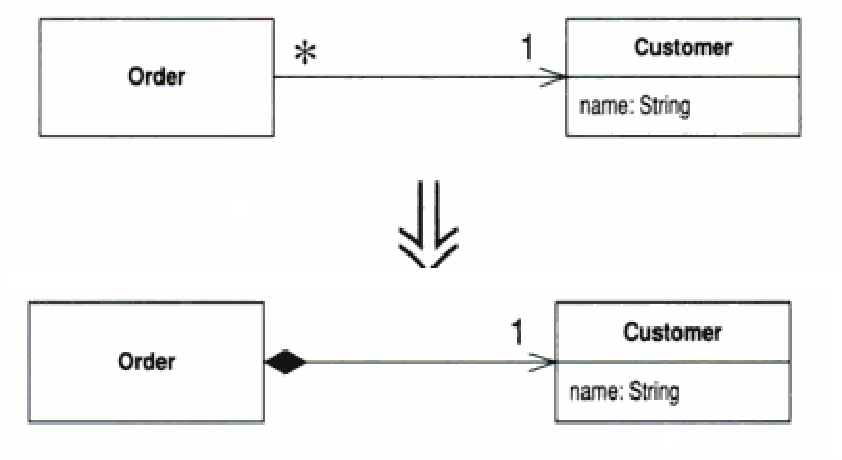
\includegraphics[scale=0.5]{4.Analysis/exemplar_refactoring.pdf}
  \end{center}
  \caption[Refactoring a reference to a value]{Refactoring a reference to a value. Taken from \cite{fowler99refactoring}[pg183].}
  \label{fig:refactoring}
\end{figure}

Before applying the refactoring, each customer may be associated with more than one order. After the refactoring, each customer should be associated with only one order. Fowler indicates that every customer associated with more than one order should be duplicated, such that one customer object exists for each order. Therefore, the migration strategy in Listing \ref{lst:refactoring} is deduced. Using this process, migration strategies were deduced for each of the refactorings that were applicable to metamodels and affected conformance.

\begin{lstlisting}[caption=Migration strategy for the refactoring in pseudo code., label=lst:refactoring]
for every customer, c
  for every order, o, associated with c
    create a new customer, d
    copy the values of c's attributes into d
  next o
	
  delete c
next c
\end{lstlisting}

The examples of metamodel evolution based on Fowler's refactorings provided additional data for deriving research requirements. Some parts of the metamodel evolutions from existing MDE projects were later found to be equivalent to Fowler's refactorings, which, to some extent, validates the above claim that evolution from object-oriented systems can be used to reason about metamodel evolution.

However, object-oriented refactorings are used to improve the maintainability of existing systems. In other words, they represent only one of the three reasons for evolutionary change defined by \cite{sjoberg93quantifying}. The two other types of change -- for addressing new requirements and facilitating interoperability with other systems -- are equally relevant for deriving research requirements, and so object-oriented refactorings alone are not sufficient for reasoning about metamodel evolution.

\subsubsection{Research collaborations}
As well as the example data located from object-oriented system, collaboration on projects using MDE with two colleagues provided several examples of evolution. A graphical editor for process-oriented programs was developed with Adam Sampson, then a Research Associate at the University of Kent, and is described in Appendix~\ref{ProcessOriented}. Additionally, the feasibility of a tool for generating story-worlds for interactive narratives was investigated with Heather Barber, then a postdoctoral researcher in this department.

In both cases, a metamodel was constructed for describing concepts in the domain. The metamodels were developed incrementally and changed over time. The collaborations with Sampson and Barber did not involve constructing model-to-model transformations, but did provide data suitable for a study of co-evolution.

The majority of the changes made in both of these projects relate to changing requirements. In each iteration, existing requirements were refined and new requirements discovered. Neither project required changes to support architectural restructuring. In addition, the work undertaken with Sampson included some changes to adapt the system for use with a different technology than originally anticipated. That is to say, the changes observed represented two of the three reasons for evolutionary change defined by \cite{sjoberg93quantifying}. 


\subsection{Summary}
This section has described the identification of example data for analysing the way in which evolution is identified and managed in the context of MDE. Example data was sought from existing MDE projects, a related domain (refactoring of object-oriented systems) and collaborative work on MDE projects (with Sampson and Barber). Eight MDE projects were located, three of which satisfied the requirements for a study of co-evolutionary changes in the context of model-driven engineering. One of the three projects, GMF, was reserved for the evaluation presented in Chapter~\ref{Evaluation}. Refactorings of object-oriented programming supplemented the data available from the existing MDE projects. Collaboration with Sampson and Barber yielded further examples of co-evolution.

Due to the lack of examples of model synchronisation, the remainder of the thesis focuses on model-metamodel co-evolution. 



\section{Analysing Existing Techniques}
\label{sec:analysing_existing_techniques}
% Having described the selection of suitable data for the analysis, we will then outline the way in which we have applied existing techniques to the data, and introduce criteria against which the effectiveness of existing techniques will be measured. 
The examples of co-evolution identified in the previous section were analysed to identify and compare existing techniques for managing co-evolution. This section discusses the results of analysing the examples; namely a deeper understanding of modelling framework characteristics that affect the management of co-evolution (Section~\ref{subsec:modelling_framework_characteristics}), and a categorisation of existing techniques for managing co-evolution (Sections~\ref{subsec:user-driven_co-evolution} and \ref{subsec:co-evolution_categorisation}) . The work presented here was published in \cite{rose09analysis,rose09enhanced}.


\subsection{Modelling Framework Characteristics}
\label{subsec:modelling_framework_characteristics}
Analysis of the co-evolution examples identified above highlighted characteristics of modern MDE modelling development environments that affect the way in which co-evolution can be managed.

\subsubsection{Model-Metamodel Separation}
In modern MDE development environments, \emph{models and metamodels are separated}. Metamodels are developed and distributed to users. Metamodels are installed, configured and combined to form a customised MDE development environment. Metamodel developers have no programmatic access to instance models, which reside in a different workspace and potentially on a different machine. Consequently, metamodel evolution occurs independently to model migration. Figure~\ref{fig:co-evo_activities} shows the activities typically involved in co-evolution. First, the metamodel developer evolves the metamodel and may create a migration strategy. Subsequently, the metamodel users discover conformance problems after installing the new version of the metamodel, and migrate their models.

\begin{figure}[htbp]
	\centering
		\includegraphics*[viewport=80 250 600 550,height=5.75cm]{4.Analysis/images/co-evo_activities.pdf}
	\caption{Co-evolution activities}
	\label{fig:co-evo_activities}
\end{figure}

Because of model and metamodel separation, co-evolution is either \emph{developer-driven} (the metamodel developer devises an executable migration strategy, which is distributed to the metamodel user with the evolved metamodel) or \emph{user-driven} (the metamodel developer provides no migration strategy). In either case, model migration occurs on the machine of the metamodel user, after and independent of metamodel evolution.


\subsubsection{Implicit Conformance}
Modern MDE development environments \emph{implicitly enforce conformance}. A model is \emph{bound} to its metamodel, typically by constructing a representation in the underlying programming language for each model element and data value. Frequently, binding is strongly-typed: each metamodel type is mapped to a corresponding type in the underlying programming language using mappings defined by the metamodel. Consequently, modelling frameworks do not permit changes to a model that would cause it to no longer conform to its metamodel. Loading a model that does not conform to its metamodel causes an error. In short, MDE modelling frameworks cannot be used to manage models that do not conform to their metamodel.

Because modelling frameworks can only load models that conform to their metamodel, user-driven migration is always a manual process, in which models are migrated without using the modelling framework. Typically then, the metamodel user can only perform migration by editing the model directly, normally manipulating its underlying representation (e.g. XMI). Model editors and model management operations, which are ordinarily integral to MDE, cannot be used to manage models that do not conform to their metamodel and hence, cannot be used during model migration.

A further consequence of implicitly enforced conformance is that modelling tools must produce models that conforms to their metamodel, and therefore, model migration cannot be decomposed. Consequently, model migration cannot be performed by combining co-evolution techniques, because intermediate steps must produce conformant models.


\subsection{User-Driven Co-Evolution}
\label{subsec:user-driven_co-evolution}
Examples of co-evolution were analysed to discover and compare existing techniques for managing co-evolution. As discussed above, the separation of models and metamodels leads to two processes for co-evolution: \emph{developer-driven} and \emph{user-driven}. Analysis of the co-evolution examples identified in Section~\ref{sec:locating_data} highlighted several instances of user-driven co-evolution. Projects conducted in collaboration with Barber and with Sampson involved user-driven co-evolution, and two of the co-evolution examples taken from the xText project were managed in a user-driven manner. This section demonstrates user-driven co-evolution using a scenario similar to one observed during the collaboration with Barber.

In user-driven co-evolution, the metamodel user performs migration by loading their models to test conformance, and then reconciling conformance problems by updating non-conformant models. The metamodel developer might guide migration by providing a migration strategy to the metamodel user. Crucially, however, the migration strategy is not executable (e.g. it is written in prose). This is the key distinction between user-driven and developer-driven co-evolution. Only in the latter does the metamodel developer provided an executable model migration strategy.  

In some cases, the metamodel user will not be provided with any migration strategy (executable or otherwise) from the metamodel developer. To perform migration, the metamodel user must determine which (if any) model elements no longer conform to the evolved metamodel, and then decide how best to change non-conformant elements to re-establish conformance.

\subsubsection{Scenario}
The following scenario demonstrates user-driven co-evolution. Mark is developing a metamodel. Members of his team, including Heather, install Mark's metamodel and begin constructing models. Mark later identifies new requirements, changes the metamodel, builds a new version of the metamodel, and distributes it to his colleagues.

After several iterations of metamodel updates, Heather tries to load one of her older models, constructed using an earlier version of Mark's metamodel. When loading the older model, the modelling framework reports an error indicating that the model no longer conforms to its metamodel. To load the older model, Heather must reinstall the version of the metamodel to which the older model conforms. But even then, the modelling framework will bind the older model to the old version of the metamodel, and not to the evolved metamodel.

Employing user-driven migration, Heather must trace and repair the loading error directly in the model as it is stored on disk. Model storage formats have typically been optimised to either reduce the size of models on disk or to improve the speed of random access to model elements. Therefore, human usability is not a key requirement for model storage formats. XMI \cite{xmi}, for example, is a standard model storage format and is regarded as sub-optimal for use by humans \cite{hutn}. Consequently, using a model storage format to perform model migration can be error-prone and tedious. When directly editing the underlying format of a model, reconciling conformance is often a slow and iterative process. For example, EMF \cite{steinberg09emf}, arguably the most widely used modelling framework, uses a multi-pass model parser and hence only reports one category of errors when a model cannot be loaded. After fixing one set of errors, another may be reported. In some cases, models are stored in a binary format and must be changed using a specialised editor, further impeding user-driven co-evolution. For example, models stored using the Connected Data Objects Model Repository (CDO)\footnote{\url{http://www.eclipse.org/cdo/}} are persisted in a relational database, which must be manipulated when non-conformant models are to be edited. 

\subsubsection{Challenges}
The above scenario highlights the two most significant challenges faced when performing user-driven co-evolution. Firstly, the underlying model representation is unlikely to be optimised for human usability and hence user-driven co-evolution is error-prone and tedious. Secondly, although conformance can be affected when a new version of a metamodel is installed, conformance problems are not reported to the user as part of the installation process. These challenges are further elaborated in the Section~\ref{sec:requirements_identification}, which identifies research requirements.

It is worth noting that the above scenario describes a metamodel with only one user. Some metamodels -- such as UML, Ecore, and MOF -- have many more users, and user-driven co-evolution would require repeated manual effort from each user. In spite of this, UML, for example, does not provide a strategy for migrating between versions of the specification, and users must infer the migration semantics from changes to the specification.

\subsection{Developer-Driven Co-Evolution Approaches}
\label{subsec:co-evolution_categorisation}
In developer-driven co-evolution, the metamodel developer provides an executable migration strategy along with the evolved metamodel. Model migration might be scheduled automatically by the modelling framework (for example when a model is loaded) or by the metamodel user.

As noted in Section~\ref{subsec:user-driven_co-evolution}, existing co-evolution research focuses on developer-driven rather than user-driven co-evolution. Several developer-driven co-evolution approaches were reviewed in Section~\ref{LitReview:ModelCoEvo}. To compare and categorise existing developer-driven co-evolution approaches, the approaches were applied -- by the author -- to the co-evolution examples identified in Section~\ref{sec:locating_data}. From this analysis and from the literature review conducted in Section~\ref{LitReview:ModelCoEvo}, three categories of developer-driven co-evolution approach were identified: \emph{manual specification}, \emph{operator-based} and \emph{inference}. This categorisation has been published in \cite{rose09analysis}. Each category is now discussed.

\subsubsection{Manual Specification}
In \emph{manual specification}, the migration strategy is encoded manually by the metamodel developer, typically using a general purpose programming language (e.g. Java) or a model-to-model transformation language (such as QVT \cite{qvt}, or ATL \cite{jouault05transforming}). The migration strategy can manipulate instances of the metamodel in any way permitted by the modelling framework. Manual specification approaches have been used to manage migration in the Eclipse GMF project \cite{gronback09emp} and the Eclipse MDT UML2 project\footnote{\url{http://www.eclipse.org/modeling/mdt/?project=uml2tools}}. Compared operator-based and inference techniques (below), manual specification permits the metamodel developer the most control over model migration.

However, manual specification generally requires the most effort on the part of the metamodel developer for two reasons. Firstly, as well as implementing the migration strategy, the metamodel developer must also produce code for executing the migration strategy. Typically, this involves integration of the migration strategy with the modelling framework (to load and store models) and possibly with development tools (to provide a user interface). Secondly, frequently occurring model migration patterns -- such as copying a model element from original to migrated model -- are not captured by existing general purpose and model-to-model transformation languages, and so each metamodel developer has to codify migration patterns in their chosen language.

\subsubsection{Operator-based}
\label{subsec:operator-based_co-evolution}
In \emph{operator-based co-evolution} techniques, a library of \emph{co-evolutionary operators} is provided. Each co-evolutionary operator specifies a metamodel evolution along with a corresponding model migration strategy. For example, the ``Make Reference Containment'' operator might evolve the metamodel such that a non-containment reference becomes a containment reference and migrate models such that the values of the evolved reference are replaced by copies. By composing co-evolutionary operators, metamodel evolution can be performed and a migration strategy can be generated without writing any code. \cite{wachsmuth07metamodel} proposes a library of co-evolutionary operators for MOF metamodels. COPE \cite{herrmannsdoerfer09cope} is an operator-based co-evolution approach for the Eclipse Modeling Framework (EMF) \cite{steinberg09emf}.

The efficacy of an operator-based co-evolution approach depends heavily on the richness of its library of co-evolutionary operators. When no operator describes the required co-evolution pattern, the metamodel developer must use another approach for performing model migration. For instance, COPE allows migration to be specified manually with a general purpose programming language when no co-evolutionary operator is appropriate. (Consequently, custom migration strategies in COPE suffer one of the same limitations as manual specification approaches: model migration patterns are not captured in the language used to specify migration strategies).

As using co-evolutionary operators to express migration require the metamodel developer to write no code, it seems that operator-based co-evolution approaches should seek to provide a large library of co-evolutionary operators, so that at least one operator is appropriate for every co-evolution pattern that a metamodel developer may wish to apply. However, as discussed in \cite{lerner00model}, a large library of operators increases the complexity of specifying migration. To demonstrate, Lerner considers moving a feature from one type to another. This could be expressed by sequential application of two operators called, for example, \texttt{delete\_feature} and \texttt{add\_feature}. However, the semantics of a \texttt{delete\_feature} operator are likely to dictate that the  values of that feature will be removed during migration and hence, \texttt{delete\_feature} is unsuitable when specifying that a feature has been moved. To solve this problem, a \texttt{move\_feature} operator could be introduced, but then the metamodel developer must understand the difference between the two ways in which moving a type can be achieved, and carefully select the correct one. Lerner provides other examples which further elucidate this issue (such as introducing a new type by splitting an existing type). As the size of the library of co-evolutionary operators grows, so does the complexity of selecting appropriate operators and, hence, the complexity of performing metamodel evolution.

Clear communication of the effects of each co-evolutionary operator (on both the metamodel and its instance models) can improve the navigability of large libraries of co-evolutionary operators. COPE, for example, provides a name, description, list of parameters and applicability constraints for each co-evolutionary operator. An example, taken from COPE's library\footnote{\url{http://cope.in.tum.de/pmwiki.php?n=Operations.MakeContainment}}, is shown below. To choose between operators, users can read descriptions (such as the one shown below) examine the source code of the operator, or try executing the operator (an undo command is provided).

\begin{quote}
\textbf{Make Reference Containment}

In the metamodel, a reference is made [into a] containment. In the model, its values are replaced by copies.

\emph{Parameters}:
\begin{itemize}
	\item \texttt{reference}: The reference
\end{itemize}

\emph{Constraints}:
\begin{itemize}
	\item The \texttt{reference} must not already be containment.
\end{itemize}
\end{quote}

Finding a balance between richness and navigability is a key challenge in defining libraries of co-evolutionary operators for operation-based co-evolution approaches. Analogously, a known challenge in the design of software interfaces is the trade-off between a rich and a concise interface \cite{bloch05apis}.

To perform metamodel evolution using co-evolutionary operators, the library of co-evolutionary operators must be integrated with tools for editing metamodels. COPE, for instance, provides integration with the EMF tree-based metamodel editor. However, some developers edit their metamodels using a textual syntax, such as Emfatic\footnote{\url{http://www.alphaworks.ibm.com/tech/emfatic}}. In general, freeform text editing is less restrictive than tree-based editing (because in the latter, the metamodel is always structurally sound whereas in the former, the text does not always have to compile). Consequently, it is not clear whether operator-based co-evolution can be used with all categories of metamodel editing tool.

\subsubsection{Inference}
\label{subsec:inference}
\label{subsec:metamodel_matching}
In \emph{inference} approaches, a migration strategy is derived from the evolved metamodel and the \emph{metamodel history}. Inference approaches can be further categorised according to the type of metamodel history used. \emph{Differencing} approaches compare and match the original and evolved metamodels, while \emph{change recording} approaches use a record of primitive changes made to the original metamodel to produce the evolved metamodel. The analysis of the evolved metamodel and the metamodel history yields a \emph{difference model} \cite{cicchetti08automating}, a representation of the changes between original and evolved metamodel. The difference model is used to infer a migration strategy, typically by using a higher-order model-to-model transformation\footnote{A model-to-model transformation that consumes or produces a model-to-model transformation is termed a higher-order model transformation.} to produce a model-to-model transformation from the difference model. \cite{cicchetti08automating} and \cite{garces09managing} describe differencing-based inference approaches. There exist no pure change recording approaches, although COPE \cite{herrmannsdoerfer09cope} uses change recording to support the specification of custom model migration strategies, and \cite{mendez10towards} suggest that change recording approach might be used to manage metamodel-transformation co-evolution.

Compared to manual specification and operator-based co-evolution approaches, inference approaches require the least amount of effort from the metamodel developer who needs only to evolve the metamodel and provide a metamodel history. However, for some types of metamodel change, there is more than one feasible model migration strategy. For example, when a metaclass is deleted, one feasible migration strategy is to delete all instances of the deleted metaclass. Alternatively, the type of each instance of the deleted metaclass could be changed to another metaclass that specifies equivalent structural features.

To select the most appropriate migration strategy from all feasible alternatives, an inference approach often requires guidance, because the metamodel changes alone do not provide enough information to correctly distinguish between feasible migration strategies. Existing inference approaches use heuristics to determine the most appropriate migration strategy. These heuristics sometimes lead to the selection of the wrong migration strategy.

Because inference approaches use heuristics to select a migration strategy, it can sometimes be difficult to reason about which migration strategy will be selected. For domains where predictability, completeness and correctness are a primary concern (e.g. safety critical or security critical systems, or systems that must undergo certification with respect to a relevant standard), such approaches are unsuitable, and deterministic approaches that can be demonstrated to produce correct, predictable results will be required. 

The two types of inference approach -- differencing and change recording -- are now compared, using an example of co-evolution, introduced below.

\paragraph{Example}
\label{subsubsec:example}
The following example was observed during the development of the Epsilon FPTC tool (summarised in Section~\ref{sec:locating_data} and described in \cite{paige08fptc}). The source code is available from EpsilonLabs\footnote{\url{http://sourceforge.net/projects/epsilonlabs/}}. Figure~\ref{fig:mm_before} illustrates the original metamodel in which a \texttt{System} comprises any number of \texttt{Block}s. A \texttt{Block} has a name, and any number of \texttt{successor} \texttt{Block}s; \texttt{predecessors} is the inverse of the \texttt{successors} reference.

\begin{figure}[htbp]
	\centering
	\subfigure[Original metamodel, prior to evolution]
	{
	    \label{fig:mm_before}
	    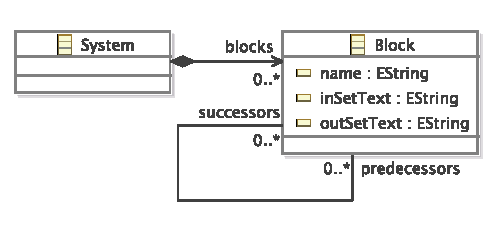
\includegraphics[scale=0.75]{4.Analysis/fptc_before.pdf}
	}
	\subfigure[Evolved metamodel with Connection metaclass]
	{
	    \label{fig:mm_after}
	    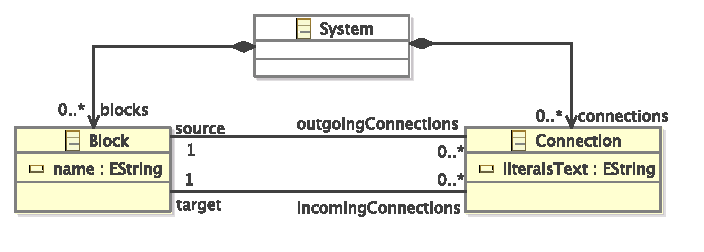
\includegraphics[scale=0.75]{4.Analysis/fptc_after.pdf}
	}
	\caption[Metamodel evolution in the Epsilon FPTC tool]{Metamodel evolution in the Epsilon FPTC tool. Taken from \cite{rose09analysis}.}
\label{fig:fptc_mm}
\end{figure}

Further analysis of the domain revealed that extra information about the relationship between \texttt{Block}s was to be captured. The evolved metamodel is shown in Figure~\ref{fig:mm_after}. The \texttt{Co\-nn\-ec\-ti\-on} class is introduced to capture the extra information via its \texttt{li\-te\-ra\-lsTe\-xt} attribute. \texttt{Block}s are no longer related directly to \texttt{Bl\-o\-ck}s, instead they are related via an instance of the \texttt{Co\-nn\-ec\-ti\-on} class. The \texttt{in\-com\-i\-ngCo\-nn\-ec\-ti\-o\-ns} and \texttt{ou\-tgo\-i\-ngCo\-nn\-ec\-ti\-o\-ns} references of \texttt{Bl\-o\-ck} are used to relate \texttt{Bl\-o\-ck}s to each other via an instance of \texttt{Co\-nn\-ec\-ti\-on}.

A model that conforms to the original metamodel (Figure~\ref{fig:mm_before}) might not conform to the evolved metamodel (Figure~\ref{fig:mm_after}). Below is a description of the strategy used by the Epsilon FPTC tool to migrate a model from original to evolved metamodel and is taken from \cite{rose09analysis}:

\begin{enumerate}
	\item For every instance, \texttt{b}, of \texttt{Block}:
		\subitem For every successor, \texttt{s}, of \texttt{b}:
			\subsubitem Create a new instance, \texttt{c}, of \texttt{Connection}.
			\subsubitem Set \texttt{b} as the \texttt{source} of \texttt{c}.
			\subsubitem Set \texttt{s} as the \texttt{target} of \texttt{c}.
			\subsubitem Add \texttt{c} to the \texttt{connections} reference of the \texttt{System} containing \texttt{b}.
	\item And nothing else changes.
\end{enumerate}

Using the example described above, differencing and change recording inference approaches are now compared. 

\paragraph{Change recording}
In change recording approaches, metamodel evolution is monitored by a tool, which records a list of primitive changes (e.g. Add class named \texttt{Connection}, Change the type of feature \texttt{successors} from \texttt{Block} to \texttt{Connection}). The record of changes may be reduced to a normal form to remove redundancy, but doing so can erase useful information. In change recording, some types of metamodel evolution can be more easily recognised than with differencing. With change recording, renaming can be distinguished from a deletion followed by an addition. With differencing, this distinction is not possible.

In general, more than one combination of primitive changes can be used to achieve the same metamodel evolution. However, when recording changes, the way in which a metamodel is evolved affects the inference of migration strategy. In the example presented above, the \texttt{outgoingConnections} reference (shown in Figure~\ref{fig:mm_after}) could have been produced by changing the name and type of the \texttt{successors} reference (shown in Figure~\ref{fig:mm_before}). In this case, the record of changes would indicate that the new \texttt{outgoingConnections} reference is an evolution of the \texttt{successors} reference, and consequently an inferred migration strategy would be likely to migrate values of \texttt{successors} to values of \texttt{out\-go\-ingCon\-nect\-ions}. Alternatively, the metamodel developer may have elected to delete the \texttt{successors} reference and then create the \texttt{out\-go\-ingCon\-nect\-ions} reference afresh. In this record of changes, it is less obvious that the migration strategy should attempt to migrate values of \texttt{successors} to values of \texttt{out\-go\-ingCon\-nect\-ions}. Clearly then, change recording approaches require the metamodel developer to consider the way in which their metamodel changes will be interpreted.

Change recording approaches require facilities for monitoring metamodel changes from the metamodel editing tool, and from the underlying modelling framework. As with operation-based co-evolution, it is not clear to what extent change recording can be supported when a textual syntax is used to evolve a metamodel. A further challenge is that the granularity of the metamodel changes that can be monitored influences the inference of the migration strategy, but this granularity is likely to be controlled by and specific to the implementation of the metamodelling language. \cite{cicchetti08thesis} discusses this issue, and proposes a normal form to which a record of changes can be reduced.


\paragraph{Differencing}
In differencing approaches, the original and evolved metamodels are compared to produce the difference model. Unlike change recording, metamodel evolution may be performed using any metamodel editor; there is no need to monitor the primitive changes made to perform the metamodel evolution. However, as discussed above, not recording the primitive changes can cause some categories of change to become indistinguishable, such as renaming versus a deletion followed by an addition.

To illustrate this problem further, consider again the metamodel evolution described above. A comparison of the original (Figure~\ref{fig:mm_before}) and evolved (Figure~\ref{fig:mm_after}) metamodels shows that the references named \texttt{successors} and \texttt{predecessors} no longer exist on \texttt{Block}. However, two other references, named \texttt{out\-go\-ingCon\-nect\-ions} and \texttt{incomingConnections}, are now present on \texttt{Block}. A differencing approach might deduce (correctly, in this case) that the two new references are evolutions of the old references. However, no differencing approach is able to determine which mapping is correct from the following two possibilities:

\begin{itemize}
	\item \texttt{successors} evolved to \texttt{incomingConnections}, and \texttt{predecessors} evolved to \texttt{outgoingConnections}.
	\item \texttt{successors} evolved to \texttt{outgoingConnections}, and \texttt{predecessors} evolved to \texttt{incomingConnections}.
\end{itemize}

The choice between these two possibilities can only made by the metamodel developer, who knows that \texttt{successors} (\texttt{predecessors}) is semantically equivalent to \texttt{outgoingConnections} (\texttt{incomingConnections}). As shown by this example, fully automatic differencing approaches cannot always infer a migration strategy that will capture the semantics desired by the metamodel developer.


\subsection{Summary}
Analysis of existing co-evolution techniques has led to a deeper understanding of modelling frameworks characteristics that are relevant for co-evolution, to the identification of user-driven co-evolution and to a categorisation of developer-driven co-evolution techniques.

Modern MDE modelling frameworks separate models and metamodels and, hence, co-evolution is a two-step process. To facilitate model migration, metamodel developers may codify an executable migration strategy and distribute it along with the evolved metamodel (developer-driven co-evolution). When no executable migration strategy is provided, models must be migrated by hand (user-driven co-evolution). Because modelling frameworks implicitly enforce conformance, user-driven co-evolution is performed by editing the underlying storage representation of models, which is error-prone and tedious.

User-driven co-evolution, which has not been explored in the literature, was observed in several of the co-evolution examples discussed in Section~\ref{sec:locating_data}. In situations where the metamodel developer has not specified or cannot specify an executable migration strategy, user-driven co-evolution is required.

Existing techniques for performing developer-driven co-evolution have been compared and categorised. The categorisation highlights a trade-off between flexibility and effort for the metamodel-developer when choosing between categories of approach, as shown in Figure~\ref{fig:developer_driven_coevo_spectrum}.


\begin{figure}[htbp]
	\centering
		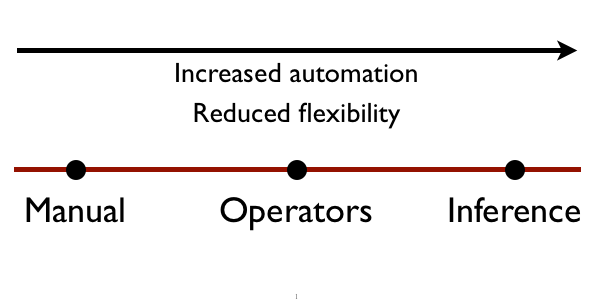
\includegraphics[width=10cm]{4.Analysis/spectrum.png}
	\caption{Spectrum of developer-driven co-evolution approaches}
	\label{fig:developer_driven_coevo_spectrum}
\end{figure}

Manual specification affords the metamodel developer more flexibility in the specification of the migration strategy, but, because languages that do not capture re-occurring model migration patterns are typically used, may require more effort. By contrast, inference approaches derive a migration strategy from a metamodel history and hence require less effort from the metamodel developer. However, an inference approach affords the metamodel developer less flexibility, and may restrict the metamodel evolution process because, for example, the order of metamodel changes affects the inference of a migration strategy. Operator-based approaches occupy the middle-ground: by restricting the way in which metamodel evolution is expressed, an operator-based approach can be used to infer a migration strategy. The metamodel developer selects appropriate operators that express both metamodel evolution and model migration. Operator-based approaches require a specialised metamodel editor, and it is not yet clear whether they can be applied when a metamodel is represented with a freeform (e.g. textual) rather than a structured (e.g. tree-based) syntax.


\section{Requirements Identification}
\label{sec:requirements_identification}
% The analysis of existing techniques will lead to requirements for our research. We will conclude the chapter by enumerating these requirements, refining the high-level research objectives from the literature review chapter into lower-level research objectives.

The analysis presented throughout this chapter has highlighted a number of challenges for identifying and managing model-metamodel co-evolution. Several factors affect and restrict the way in which co-evolution is performed in practice. The way in which modelling frameworks are implemented affect the ways in which the impact analysis and propagation of metamodel changes can be performed. Existing co-evolution approaches are developer-driven rather than user-driven (i.e. assume that the metamodel developer will provide a migration strategy), which was not the case for several of the examples identified in Section~\ref{sec:locating_data}. Additionally, the languages used to specify model migration vary over existing co-evolution approaches, which inhibits the conceptual and practical re-use of model migration patterns. This section contributes requirements for structures and processes that seek to address these challenges.

Below, the thesis requirements are presented in three parts. The first identifies requirements that seek to extend and enhance support for managing model and metamodel co-evolution with modelling frameworks. The second summarises and identifies requirements for enhancing the user-driven co-evolution process discussed in Section~\ref{subsec:user-driven_co-evolution}. Finally, the third identifies requirements that seek to improve the spectrum of existing developer-driven co-evolution techniques.


\subsection{Explicit conformance checking}
Section~\ref{subsec:modelling_framework_characteristics} discussed characteristics of modelling frameworks relevant to managing co-evolution. Because modelling frameworks typically enforce model and metamodel conformance implicitly, they cannot be used to load non-conformant models. Consequently, user-driven co-evolution involves editing a model in its storage representation, which is error-prone and tedious, because human usability is not normally a key requirement for model storage representations. Furthermore, modelling frameworks that implicitly enforce conformance understandably provide little support for explicitly checking the conformance of a model with other metamodels (or other versions of the same metamodel). As discussed in Section~\ref{subsec:modelling_framework_characteristics}, explicit conformance checking is useful for determining whether a model needs to be migrated (during the installation of a newer version of its metamodel, for example).

Therefore, the following requirement was derived: \emph{This thesis must investigate the extension of existing modelling frameworks to support the loading of non-conformant models and conformance checking of models against other metamodels.}


%conformance isn't checked during metamodel installation, so conformance problems may not be discovered as soon as they arise


\subsection{User-driven co-evolution}
When a metamodel change will affect conformance in only a small number of models, a metamodel developer may decide that the extra effort required to specify an executable migration strategy is too great, and prefer a user-driven co-evolution technique. Section~\ref{subsec:user-driven_co-evolution} introduced -- and highlighted several challenges for -- user-driven co-evolution.

Because modelling frameworks typically cannot be used to load models that do not conform to their metamodel, user-driven co-evolution involves editing the storage representation of a model. As discussed above, model storage representations are typically not optimised for human use and hence user-driven co-evolution can be error-prone and time consuming. When a multi-pass parser is used to load models (as is the case with EMF), user-driven co-evolution is an iterative process, because not all conformance errors are reported at once.

Therefore, the following requirement was derived: \emph{This thesis must demonstrate a user-driven co-evolution process that enables the editing of non-conformant models without directly manipulating the underlying storage representation and provides a conformance report for the original model and evolved metamodel.}


\subsection{Developer-driven co-evolution}
The comparison of developer-driven co-evolution techniques (Section~\ref{subsec:co-evolution_categorisation}) highlights variation in the languages used for codifying model migration strategies. More specifically, the model migration strategy languages varied in their scope (general-purpose programming languages versus model transformation languages) and category of type system. Furthermore, the amount of processing performed when executing a model migration strategy also varied: some techniques only load a model, execute the model migration strategy using an existing execution engine and store the model, while others perform significant processing in addition to the computation specified in the model migration strategy. COPE, for example, transforms models to a metamodel-independent representation before migration is executed, and back to a metamodel-specific representation afterwards.

Of the three categories of developer-driven co-evolution technique identified in Section~\ref{subsec:co-evolution_categorisation}, only manual specification (in which the metamodel developer specifies the migration strategy by hand) always requires the use of a migration strategy language. Nevertheless, both operator-based and inference approaches might utilise a migration strategy language in particular circumstances. Some operator-based approaches, such as COPE, permit manual specification of a model migration strategy when no co-evolutionary operator is appropriate. For describing the effects of co-evolutionary operators, the model migration part of an operator could be described using a model migration strategy language. When an inference approach suggests more than one feasible migration strategy, a migration strategy language could be used to present alternatives to the metamodel developer. To some extent then, the choice of model migration strategy language influences the efficacy of all categories of developer-driven co-evolution approach.  

Given the variations in existing model migration strategy languages and the influence of those languages on developer-driven co-evolution, the following requirement was derived: \emph{This thesis must compare and evaluate existing languages for specifying model migration strategies.}

As discussed in Section~\ref{subsec:co-evolution_categorisation}, existing manual specification techniques do not provide model migration strategy languages that capture patterns specific to model migration. Developers must re-invent solutions to commonly occurring model migration patterns, such as copying an element from the original to the migrated model. In some cases, manual specification techniques require the developer to implement, in addition to a migration strategy, infrastructure features for loading and storing models and for interfacing with the metamodel user. 

Devising a domain-specific languages or DSL (discussed in Chapter~\ref{LiteratureReview}) is one mechanism for capturing re-occurring patterns. Executable DSLs are often used for performing model management in contemporary model-driven development environments. DSLs are provided by model-to-model (M2M) transformation tools such as ATL \cite{jouault05transforming}, VIATRA \cite{VIATRA}, workflow architectures such as oAW\footnote{\url{http://www.eclipse.org/workinggroups/oaw/}}, and model-to-text (M2T) transformation tools such as MOFScript \cite{oldevik05toward}.

Given the apparent appropriateness of a domain-specific language for specifying model migration and that no common language for specifying migration has yet been devised, the following requirement was derived: \emph{This thesis must implement and evaluate a domain-specific language for specifying and executing model migration strategies, comparing it to existing languages for specifying model migration strategies.}

\section{Chapter Summary}
The literature review performed in Chapter~\ref{LiteratureReview} identified several types of evolution that occur in MDE projects, including model refactoring, synchronisation and co-evolution. Although several papers propose structures and processes for managing evolution in MDE, little work has considered the way in which MDE artefacts evolve in practice. The work described in this chapter has investigated evolution in existing MDE projects, culminating in a deeper understanding of the conceptual and technical issues faced when identifying and managing co-evolution. Furthermore, the analysis has facilitated the derivation of requirements for structures and processes that will address several of the challenges to identifying and managing co-evolution today.

Examples of co-evolution were identified from real-world MDE projects, and supplementary data was located by examining a related area (refactoring in object-oriented systems) and from collaborative work on two projects using MDE. The examples were used to understand how co-evolution is performed in practice, and led to the identification of user-driven co-evolution. Furthermore, the examples were used to analyse and categorise existing approaches to managing co-evolution.

Examining the co-evolution examples and applying existing co-evolution tools to the examples led to several observations. Firstly, modelling frameworks restrict the way in which co-evolution can be identified and managed. Secondly, user-driven co-evolution (in which models are migrated without an executable strategy) occurs in practice, but no existing co-evolution tools provide support for it. Finally, the variation of languages used for specifying model migration inhibits the re-use of commonly occurring patterns.

From the analysis performed in this chapter, requirements for the implementation phase of the thesis were formulated. The structures and process developed to approach those requirements are described in Chapter~\ref{Implementation}, and seek to alleviate the restrictions of modelling frameworks, to improve and support user-driven co-evolution (which is currently error-prone and tedious), and to provide a common language for specifying model migration.

